\chapter{Gebruikersaspecten}
\label{ch:gebruikersaspecten}
\section{High-Level requirements}
De applicatie kan gebruikt worden door twee type actoren. Een normale gebruiker (student) en een docent. De docent is een speciaal geval van een normale gebruiker met extra rechten, maar heeft ook dezelfde rechten als een normale gebruiker.
\subsection{Functionele requirements}
\subsubsection{Login}
\begin{itemize}
	\item De gebruiker kan zich inloggen via het UGent CAS-systeem of via een dummy systeem dat dit nabootst.
\end{itemize}
\subsubsection{Dashboard}
\begin{itemize}
	\item De gebruiker kan een video selecteren op het dashboard.
    \item De gebruiker kan een videobestand uploaden in de applicatie
 	\item De docent kan gebruikers koppelen aan een video.
 	\item De docent kan een deadline instellen van een video.
 	\item De docent kan een label toevoegen aan een video.
 	\item De docent kan groepjes van gebruikers aanmaken.
 	\item De docent kan de video's filteren per thema of categorie.
 	\item De docent kan quick comments beheren.
 	\item De docent kan quick comments koppelen aan een video.
 	\item De docent kan het niveau van toegankelijkheid voor de annotaties van een bepaalde video instellen.
	\item De docent kan voor een video of meerdere video's de annotaties exporteren.
 	\item De docent kan een .csv file uploaden.

\end{itemize}
\subsubsection{Video interactief}
\begin{itemize}
	\item De gebruiker kan op een specifiek moment een annotatie plaatsen.
	\item De gebruiker kan op een annotatie klikken om naar dat punt in de video te springen waarop de annotatie geplaatst is.
	\item De gebruiker kan een quick comment toevoegen op het huidige tijdstip van de video.
	\item De docent kan een video afspelen of pauzeren.
	\item De docent kan zoeken tussen alle annotaties van een bepaalde video.
\end{itemize}
\subsection{Niet-functionele requirements}
\begin{itemize}
 \item De website moet gebruiksvriendelijk zijn. De website moet eenvoudig te begrijpen zijn voor onervaren computergebruikers.
 \item Aangezien dat de video's vertrouwelijke inhoud kunnen bevatten, moet hiervoor de nodige beveiliging voorzien worden.
 \item Tijdens het typen van een annotatie zou de informatie voortdurend automatisch opgeslagen moeten worden zodat er geen werk verloren gaat. 
\end{itemize}

\subsection{Identificatie}
Gebruikers worden herkend aan de hand van hun UGent credentials. De applicatie kan alleen maar gebruikt worden door personen die verbonden zijn aan de UGent.

\section{Use case diagram}
Figuur 2.1 toont het use case diagram. Het systeem kent slechts 2 actoren: een normale gebruiker en een docent. Aangezien er een poging werd gedaan om het UGent CAS loginsysteem te gebruiken, bestaat er geen actie 'registreren'.
\begin{figure}
    \centering
        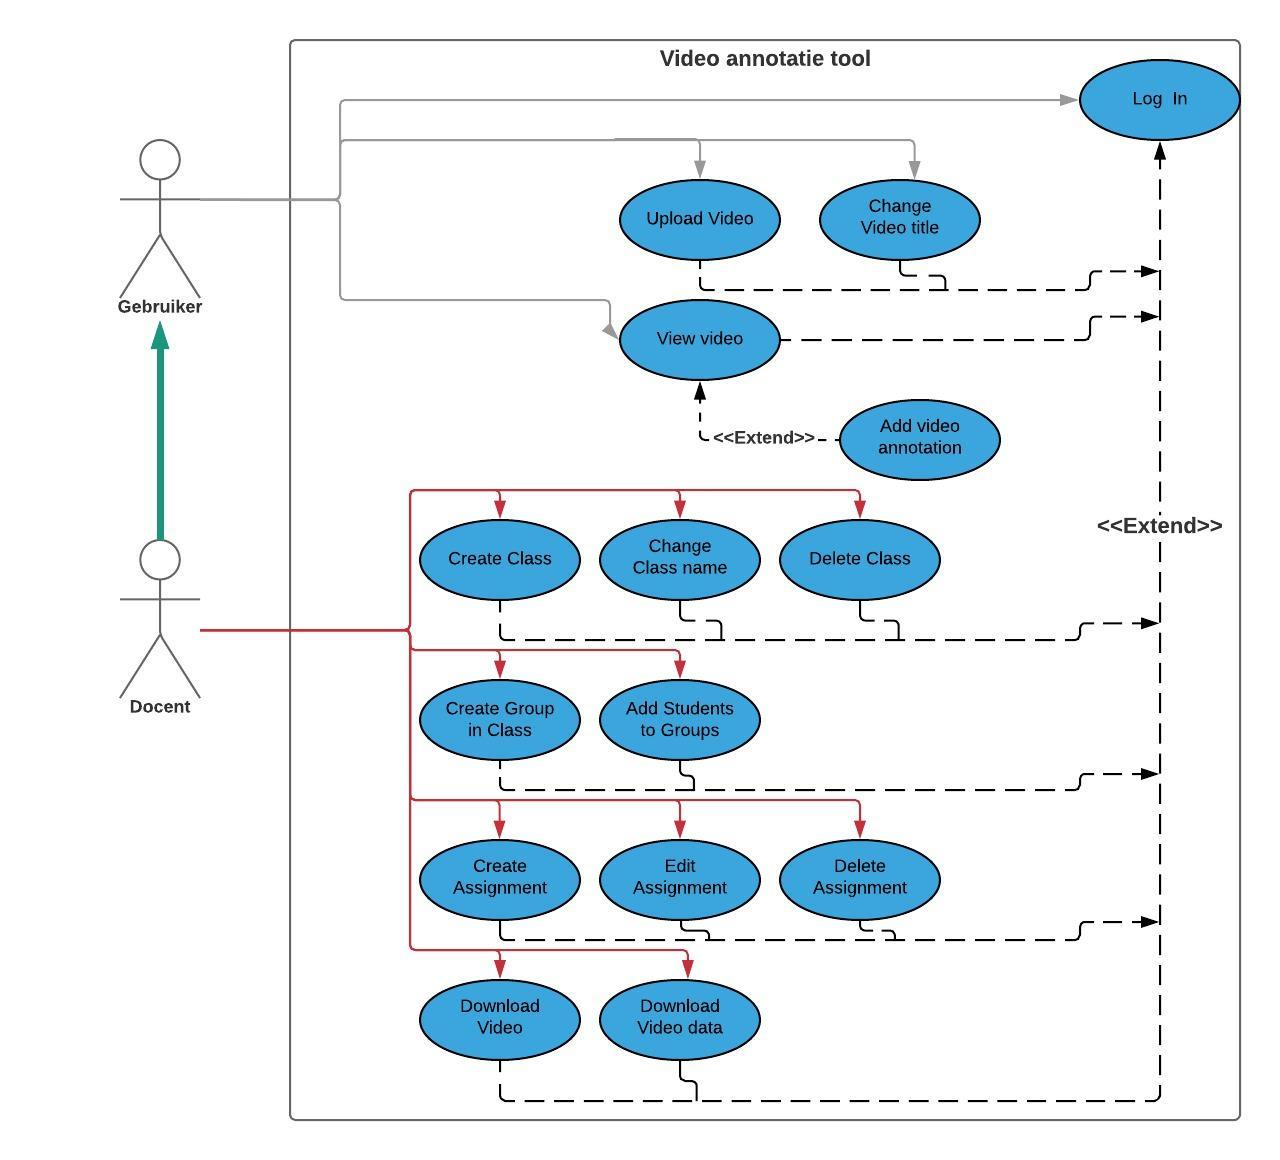
\includegraphics[width=\textwidth]{usecase2}
    \caption{Het use case diagram}
\end{figure}
\pagebreak
\section{Use cases}
\subsection{Upload video}
\begin{usecase}
	\addtitle{Use Case 1}{Upload video}
	\addfield{Actor:}{Gebruikers en docenten}
	\addfield{Trigger:}{De gebruiker selecteert de optie om een video te uploaden}
	\addscenario{Precondities:}{
		\item[-] De gebruiker is ingelogd (Log in use case)
		\item[-] Er is een opdracht aangemaakt door de docent (Create assignment use case)
	}
	\addscenario{Postcondities:}{
		\item[-] De video is geüpload en zichtbaar voor de gebruiker zelf en voor de gebruikers met wie de video gedeeld is
	}
	\addscenario{Basis flow:}{
		\item Het systeem toont het scherm waarop een video kan geüpload worden
		\item De gebruiker selecteert lokaal een video file
		\item Het systeem controleert of het om een video file gaat
		\item De gebruiker geeft de video een titel
		\item De gebruiker selecteert de bijhorende opdracht
		\item De gebruiker bevestigt de upload
		\item Het systeem slaat de video en bijhorende info op
		\item Het systeem toont de geüploade video
	}
	\addscenario{Alternatieve flow:}{
		\item[3a.] De gebruiker selecteerde een file dat geen video format is
		\begin{enumerate}
			\item[3a.1] Het systeem toont een foutboodschap en vraagt om de juist file te selecteren
			\item[3a.2] Terug naar stap 2
		\end{enumerate}      
	}
\end{usecase}
\pagebreak
\subsection{Add video annotation}
\begin{usecase}
	\addtitle{Use Case 2}{Add video annotation}
	\addfield{Actor:}{Gebruikers en docenten}
	\addfield{Trigger:}{De gebruiker selecteert een video}
	\addscenario{Precondities:}{
		\item[-] De gebruiker is ingelogd (Log in use case)
		\item[-] De gebruiker is een video aan het bekijken (View video use case)
	}
	\addscenario{Postcondities:}{
		\item[-] Een annotatie is opgeslagen voor een video
	}
	\addscenario{Basis flow:}{
		\item De gebruiker pauzeert de video stream
		\item De gebruiker geeft de tekst voor de annotatie in
		\item De gebruiker bevestigt de annotatie
		\item Het systeem slaat de annotatie met bijhorende timestamp op en geeft deze weer 
	}
	\addscenario{Alternatieve flow:}{
		\item[1a.] De video wordt niet gepauzeerd
		\begin{enumerate}
			\item[1a.1] De gebruiker selecteert een quick comment annotatie
			\item[1a.2.] Ga verder met stap 4
		\end{enumerate} 
		\item[2a.] Het gaat om een Drop down menu annotatie
		\begin{enumerate}
			\item[2a.1] De gebruiker selecteert de juist optie in de dropdown
			\item[2a.2] De gebruiker geeft bijhorende tekst in voor de annotatie
			\item[2a.3] Ga verder met stap 3
		\end{enumerate} 
	}
\end{usecase}
\pagebreak
\subsection{Create class}
\begin{usecase}
	\addtitle{Use Case 3}{Create class}
	\addfield{Actor:}{Docenten}
	\addfield{Trigger:}{De gebruiker selecteert de optie om een klas aan te maken}
	\addscenario{Precondities:}{
		\item[-] De gebruiker is ingelogd (Log in use case)
	}
	\addscenario{Postcondities:}{
		\item[-] Een nieuwe klas is aangemaakt met bijhorende gebruikers
	}
	\addscenario{Basis flow:}{
		\item Het systeem toont een pop-up waarin de gebruiker een klas kan aanmaken
		\item De gebruiker selecteert lokaal een .csv file met gebruikers
		\item Het systeem controleert of het een .csv file is en of deze correcte formattering gebruikt
		\item De gebruiker geeft de klas een naam
		\item De gebruiker bevestigt het aanmaken
		\item Het systeem slaat de klas en bijhorende gebruikers op
	}
	\addscenario{Alternatieve flow:}{
	        \item [3a.] Het .csv bestand heeft geen geldig formaat
	        \begin{enumerate}
	         \item [3a.1] Het systeem toont een gepaste melding
	         \item [3a.2] Keer terug naar stap 2
	        \end{enumerate}

	
	
	}
\end{usecase}
\pagebreak
\subsection{Create assignment}
\begin{usecase}
	\addtitle{Use Case 6}{Create assignment}
	\addfield{Actor:}{Docenten}
	\addfield{Trigger:}{De gebruiker selecteert de optie om een opdracht aan te maken
	}
	\addscenario{Precondities:}{
		\item[-] De gebruiker is ingelogd (Log in use case)
	}
	\addscenario{Postcondities:}{
		\item[-] Een nieuwe opdracht is aangemaakt
	}
	\addscenario{Basis flow:}{
		\item Het systeem toont een pop-up waarin de gebruiker een opdracht kan aanmaken
		\item De gebruiker geeft de opdracht een naam
		\item De gebruiker activeert de gewenste annotaties en vult de juiste bijhorende waarden in
		\item De gebruiker geeft aan of de annotaties privé zijn of niet
		\item De gebruiker selecteert voor welke klas of groep de opdracht is
		\item De gebruiker geeft aan wie de uploads mag doen (docent of gebruiker)
		\item De gebruiker geeft mogelijk een deadline mee
		\item Het systeem controleert de data
		\item Het systeem maakt de opdracht aan en slaat de data op
		\item Het systeem toont een overzicht van alle opdrachten
	}
	\addscenario{Alternatieve flow:}{
		\item[8a.] De data is niet volledig
		\begin{enumerate}
			\item[8a.1] Het systeem toont een foutboodschap
			\item[8a.2] De gebruiker overloopt opnieuw vanaf stap 2
		\end{enumerate} 
	}
\end{usecase}
\pagebreak
\subsection{Download video data}
\begin{usecase}
	\addtitle{Use Case 8}{Download video data}
	\addfield{Actor:}{Docenten}
	\addfield{Trigger:}{De gebruiker selecteert de optie om de video data te downloaden
	}
	\addscenario{Precondities:}{
		\item[-] De gebruiker is ingelogd (Log in use case)
		\item[-] De gebruiker is een video aan het bekijken (View video use case)
	}
	\addscenario{Postcondities:}{
		\item[-] De gebruiker heeft een lokale versie van de verschillende annotaties van de video	
	}
	\addscenario{Basis flow:}{
		\item Het systeem pauzeert de video
		\item Het systeem vraagt of de gebruiker zeker is
		\item De gebruiker bevestigt
		\item Het systeem genereert de data file
		\item Het systeem start een download van die file naar de computer van de gebruiker
	}
	\addfield{Alternatieve flow:}{/
	}
\end{usecase}
\pagebreak




\section{Backlog}
De volgende lijst stelt de product backlog voor, inclusief volgende attributen: extra uitleg, de prioriteit, de complexiteit, in welk sprint deze feature afgewerkt is en eventueel extra opmerkingen.

\begin{itemize}
\setlength\itemsep{2em}
 \item Als een gebruiker wil ik een video kunnen uploaden (\textbf{Sprint 1})
        
        \textbf{Uitleg} Het uploaden van een video is \'e\'en van de basisfunctionaliteiten.
        
        \textbf{Prioriteit}: 5/5  \textbf{Complexiteit}: 3/5
        
 \item Als een gebruiker wil ik een video kunnen bekijken (\textbf{Sprint 1})

        \textbf{Uitleg}: Het bekijken van een video is \'e\'en van de basisfunctionaliteiten.

        \textbf{Prioriteit}: 5/5 \textbf{Complexiteit}: 2/5
        
 \item Als een gebruiker wil ik annotaties kunnen plaatsen op een video (\textbf{Sprint 2})

        \textbf{Uitleg}: Het toevoegen van annotaties is \'e\'en van de basisfunctionaliteiten.

        \textbf{Prioriteit}: 5/5 \textbf{Complexiteit}: 3/5
 \item Als een gebruiker wil ik quick annotations toevoegen aan een video (\textbf{Sprint 2})
        
        \textbf{Uitleg}: Het toevoegen van quick annotations is een uitbreiding op de normale annotaties.
            \textbf{Prioriteit}: 4/5 \textbf{Complexiteit}: 1/5

            
 \item  Als een gebruiker wil ik naar een punt in de video springen waar een annotatie staat zodat ik de annotatie kan bekijken (\textbf{Sprint 2})

        \textbf{Uitleg}: Een gebruiker wil een eenvoudige manier om het filmpje af te spelen op de plaats waar een annotatie geplaatst is

        \textbf{Prioriteit}: 3/5 \textbf{Complexiteit}: 1/5
 \item Als een gebruiker wil ik een dashboard zodat ik een overzicht heb van mijn taken en video's (\textbf{Sprint 2})

        \textbf{Uitleg}: Het dashboard is de eerste pagina dat getoond wordt wanneer een gebruiker inlogt. Deze pagina moet direct een overzicht bieden van de nog te maken taken, en video's die kunnen bekeken worden

        \textbf{Prioriteit}: 4/5 \textbf{Complexiteit}: 3/5
 \item Als een docent wil ik klasgroepen importeren uit een .csv bestand zodat ik een overzicht heb van mijn studenten (\textbf{Sprint 2})

        \textbf{Uitleg}: Aangezien het UGent CAS systeem uiteindelijk niet op de applicatie is aangesloten, kunnen de klasgroepen niet rechtstreeks vanuit dit systeem gehaald worden. De applicatie laat toe een .csv bestand up te loaden die een .csv export van Minerva nabootst zodat hieruit klasgroepen kunnen gemaakt worden.

        \textbf{Prioriteit}: 3/5 \textbf{Complexiteit}: 4/5
 \item  Als een gebruiker wil ik taken bekijken zodat ik daar een video voor kan uploaden (\textbf{Sprint 3})
        
        \textbf{Uitleg}: De gebruiker moet een overzicht hebben van zijn taken om te weten waar hij een video kan uploaden
        
        \textbf{Prioriteit}: 3/5 \textbf{Complexiteit}: 3/5
 \item Als een gebruiker wil ik kunnen inloggen zodat ik gebruik kan maken van de applicatie (\textbf{Sprint 3})

        \textbf{Uitleg}: Een geldig UGent email-adres hebben is verplicht om gebruik te kunnen maken van de applicatie. Indien de gebruiker een geldig UGent email-adres heeft kan de gebruiker inloggen op de applicatie.


        \textbf{Prioriteit}: 5/5 \textbf{Complexiteit}: 4/5

        \textbf{Opmerking}: Deze feature werd ook al eens in sprint 1 opgenomen, maar er was onvoldoende kennis over het UGent Cas systeem om de implementatie te starten

        
        
\end{itemize}


